\documentclass[11pt, oneside]{article}   	% use "amsart" instead of "article" for AMSLaTeX format
\usepackage{geometry}                		% See geometry.pdf to learn the layout options. There are lots.
\geometry{letterpaper}                   		% ... or a4paper or a5paper or ... 
\usepackage[parfill]{parskip}    		% Activate to begin paragraphs with an empty line rather than an indent
\usepackage{graphicx}				% Use pdf, png, jpg, or eps§ with pdflatex; use eps in DVI mode
								% TeX will automatically convert eps --> pdf in pdflatex		
\usepackage{caption}
\usepackage{pifont,natbib,geometry,fleqn}
\usepackage{amsmath,amssymb,amsfonts,amsthm,epsf,epsfig}
\usepackage{array,color,multirow}
\usepackage{mathtools}
\usepackage{hyperref}

%SetFonts

%SetFonts


\title{gr-MRI User Guide}
\author{Chris Hasselwander, Will Grissom}
\date{October, 21 2015}

\begin{document}

\newpage
\tableofcontents
\newpage

\section{Necessary Hardware}
In order to construct the USRP1 based MRI spectrometer as we have, you will need the following hardware:
\begin{enumerate}
	\item Ettus Research:
	\begin{itemize}
		\item (2x) \textbf{Ettus Research USRP1} (\$707 ea.): \url{http://www.ettus.com/product/details/USRPPKG}
		\begin{description}
			\item[Note:] This package comes with a USB cable, power supply, and 2 SMA bulkhead cables
		\end{description}
		\item (4x) \textbf{Ettus Research LFRX} (\$76 ea.): \url{http://www.ettus.com/product/details/LFRX}
		\item (4x) \textbf{Ettus Research LFTX} (\$76 ea.): \url{http://www.ettus.com/product/details/LFTX}
		\item (?6x) \textbf{SMA Bulkhead Cable} (\$20 ea): \url{http://www.ettus.com/product/details/SMA-Bulkhead}
	\end{itemize}
	\item Digikey (amp circuit):
	\begin{itemize}
		\item \textbf{item 1}
		\item \textbf{item 2}
		\item \textbf{item 3}
	\end{itemize}
	\item Miscellaneous:
	\begin{itemize}
		\item SMA-SMA cable to connect clocks
		\item (2x) short SMA-SMA cable for internal loopbacks
		\item misc electrical wires
		\item 8x BNC to SMA connectors (female to male)
	\end{itemize}
\end{enumerate}

\section{Setup}
\subsection{Hardware Setup}
\subsubsection{Synchronize the two USRP1s}

\indent The clocks on the different USRP1s may be slightly different, and without synchronization pulses sent out of both boards will shift relative to one another in time.  It is necessary to syncrhonize the on board clocks to enable sequenced operation.  The following instructions have been slightly modified from the 
\color{blue}
\href{https://gnuradio.org/redmine/projects/gnuradio/wiki/USRPClockingNotes\#Synchronizing-multiple-USRP1s}{GNU Radio clock synchronization instrucitons}.
\color{black}

\begin{enumerate}
	\item Decide which board will be the master, and which will be the slave.  The gr-MRI package assumes that the RF board will serve as the master, so you should do the same.
	\item For the master clock board:
	\begin{enumerate}
		\item Solder an SMA connector into J2002. This is the master clock output. Be careful when soldering the SMA connector so you don't break the delicate trace from J2002 to R2028.
	\end{enumerate}
	\item For the slave boards:
	\begin{enumerate}
		\item Solder an SMA connector into J2001. This is the clock input. Be careful when soldering the SMA connector so you don't break the delicate trace from J2001 to C927.
		\item Move R2029 to R2030. This disables the onboard clock. R2029/R2030 is a 0-ohm resistor.
		\item Move C925 to C926.
		\item Remove C924.
		\item If you want to chain another USRP device off of this one, you can use J2002 to provide a clock out
	\end{enumerate}
	\item To synchronize the clocks, simply connect the connectors that were soldered on.
\end{enumerate}



\subsubsection{Attach LFTX and LFRX daughterboards in appropriate motherboard slots}

\indent Insert the LFTX and LFRX daughterboards into the appropriate slots on the motherboard according to  Figure~\ref{fig:motherboard_img} below.  The slots are also labeled \textit{TX\_A, TX\_B, RX\_A, RX\_B} on the motherboard.  Screw the daughterboards so they are secure.  \textbf{For this guide I will refer to ports as \emph{m-board d-board\_slot\_channel}.} \textbf{ So for example, The RX\_B channel for the RF board's RX\_A slot would be \emph{RF RX\_A\_B}.}

\begin{figure}[!ht]
\begin{center}
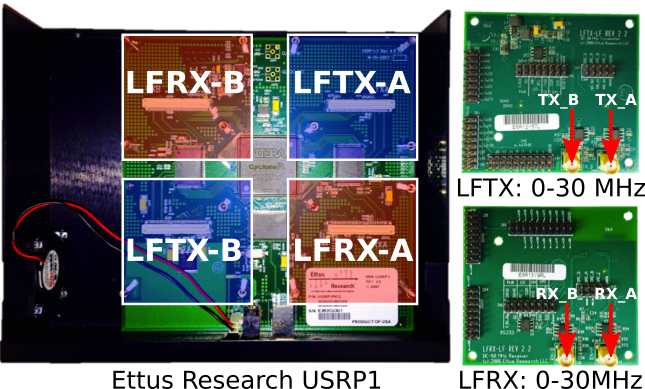
\includegraphics[width = \textwidth,trim=0 0 0 0,clip=false]{motherboard_img.png}
\caption{\textcolor{black}{Image of Ettus Research USRP1 motherboard, LFTX, and LFRX daughterboard placement}}
\label{fig:motherboard_img}
\end{center}
\end{figure}

\subsection{Build "amplifier" circuit for TXE pathway}

\indent Come back to this guy later

\subsection{Connect SMA bulkhead cables to enclosure output/input slots and connect internal feedback cables}

\begin{enumerate}
	\item Connect the following ports to the output/input holes in the USRP1 enclosure.  It doesn't matter which holes to connect to, but you may want to write which slot corresponds to which daughterboard or desired signal.
	\begin{itemize}
		\item RF TX\_A\_A \textit{(RF Channel 1 Signal Out)}
		\item RF RX\_A\_A \textit{(RF Signal RX)}
		\item RF Master Clock - connect to DC Slave Clock
		\item RF TX\_B\_A \textit{(Synchronizing Pulse)}
		\item DC TX\_A\_A \textit{(Z Gradient)}
		\item DC TX\_A\_B \textit{(Y Gradient)}
		\item DC TX\_B\_B \textit{(X Gradient)}
		\item DC Slave Clock - connect to RF Master Clock
		\item DC RX\_A\_A \textit{(RF sync pulse input)}
	\end{itemize}
	\item Connect the following internal feedback loops:
	\begin{itemize}
		\item Connect RF TX\_A\_B to RF RX\_B\_A \textit{(Readout Window)}
	\end{itemize}
	\item Special Connections:
	\begin{itemize}
		\item Connect DC TX\_B\_A through TXE amplifier output 1 to output slot \textit{(TXE pulse)}
		\item Connect DC TX\_B\_A through TXE amplifier output 2 to DC RX\_B\_A \textit{(sync feedback pulse)}
	\end{itemize}
\end{enumerate}

\subsection{Connect USRP1 outputs and inputs to external hardware}
\indent RF amplifiers, TX/RX coil, Preamplifier, Gradient Amplifiers, etc.

\section{Software Setup}
\subsection{GNU Radio Setup}

\indent Download and install GNU Radio and all of its dependencies following the instructions at \url{https://gnuradio.org/redmine/projects/gnuradio/wiki/UbuntuInstall}.  This will take some time.


\subsection{Downloading and Installing gr-MRI}

\indent To download the current version of the gr-MRI package on Linux machine:
\begin{enumerate}
	\item Open a new terminal and navigate to the directory in which you want to save gr-MRI.
	\item type \texttt{git init} 
	\item type \texttt{git remote add origin ssh git@bitbucket.org:wgrissom/gnuradio-mri.git}
	\item type \texttt{git clone git@bitbucket.org:wgrissom/gnuradio-mri.git}
\end{enumerate}

\indent To add the gr-MRI custom blocks for use in GNU Radio:
\begin{enumerate}
	\item Open a terminal and navigate to \texttt{gnuradio-mri/gr\_3.7/gr-MRI}, and type:
	\item \texttt{mkdir build}
	\item \texttt{cd build}
	\item \texttt{cmake ../}
	\item \texttt{make}
	\item \texttt{sudo make install}
	\item \texttt{sudo ldconfig}
\end{enumerate}

\subsection{Editing GNU Radio settings for stock sequences}
\indent You will need to change some of the settings within each of the GNU Radio flowgraphs to allow them to work with your USRP1s.  The files to edit are called \textit{spin\_echo.grc,gradient\_echo.grc,calibration.grc}.
\begin{itemize}
	\item connect the two USRP1 radios that you plan to use for open a terminal window and type \texttt{uhd\_find\_devices} to make sure that your computer can see the devices.  The function will return the serial numbers of the devices.  Look on the motherboard of each radio to see which serial number corresponds to which radio (RF or DC).
	\item Open the \texttt{.grc} file and find the blocks titled "USRP sink." The topmost block is always the RF radio sink, and the block below it is the DC radio sink for the files in gr-MRI.
	\item Double click the top USRP sink to open the settings, shown in Figure~\ref{fig:usrpsink}, and replace the serial number written in the "Device Address" to the serial number of your RF radio.
	
	\begin{figure}[!ht]
	\begin{center}
	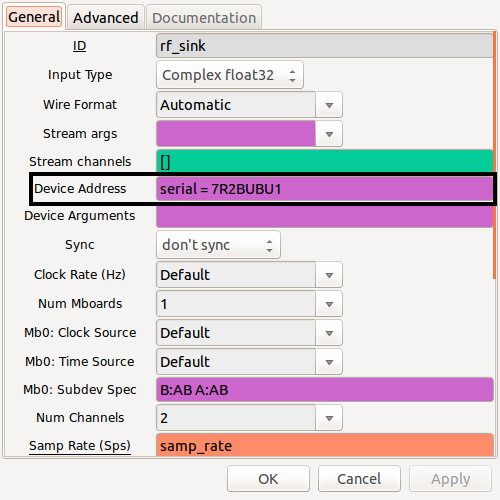
\includegraphics[width = .65\textwidth,trim=0 0 0 0,clip=false]{usrpsink_settings.png}
	\caption{\textcolor{black}{Image of Ettus Research USRP1 motherboard, LFTX, and LFRX daughterboard placement}}
	\label{fig:usrpsink}
	\end{center}
	\end{figure}
	
	\item Repeat the same procedure for the bottom USRP Sink
	
\end{itemize}

\section{Using gr-MRI}
\subsection{Overview}



\subsection{RF Pulse Calibration}



\subsection{Gradient Calibration}



\subsection{Stock Imaging Sequences}
\subsubsection{Slice Selective Gradient Echo: \textit{gradecho.py}}



\subsubsection{Slice Selective Spin Echo: \textit{slicespin.py}}




\subsubsection{Slice Selective Inversion Recovery: \textit{invrecov.py}}

\end{document}  








